% author Truong Nhan Nguyen
% created in 1/1/2022
\documentclass[tikz, border=10pt]{standalone}

\usepackage{tikz}
\usetikzlibrary{arrows}
\usepackage{amsmath, amsfonts, mathtools, amssymb}
\usepackage{mathpazo}

\tikzstyle{every picture} += [remember picture]
\tikzstyle{every node} = [rounded corners, inner sep=3pt]

\begin{document}
    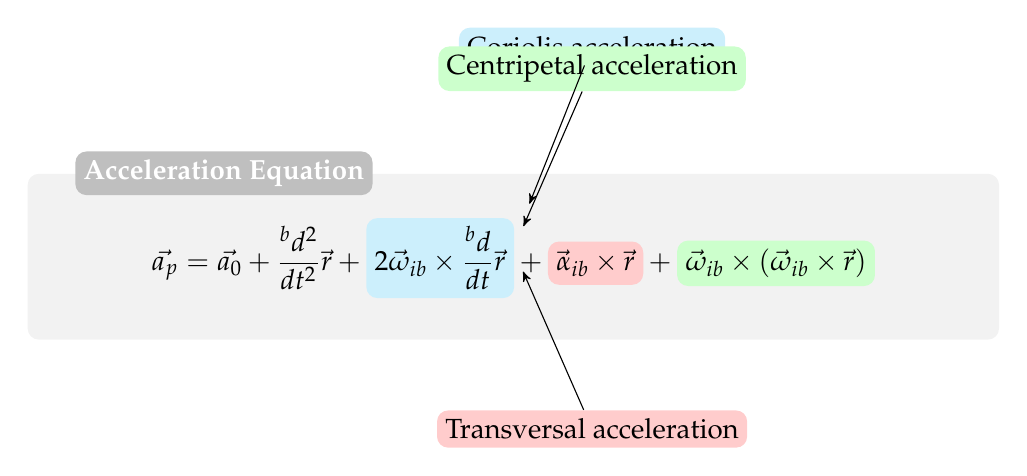
\begin{tikzpicture}
        \node[fill=gray!10, inner ysep=15pt] (eq) {
            \begin{minipage}{\textwidth}
                \begin{equation*}
                    \vec{a_p} = \vec{a_0} + \dfrac{{}^bd^2}{dt^2}\vec{r} + 
                    \tikz[baseline]{
                        \node[fill=cyan!20, anchor=base] (t1) { $2\vec{\omega}_{ib}\times\dfrac{{}^bd}{dt}\vec{r}$
                        };
                    } + 
                    \tikz[baseline]{
                        \node[fill=red!20, anchor=base] (t2) {
                            $\vec{\alpha}_{ib}\times\vec{r}$
                        };
                    } + 
                    \tikz[baseline]{
                        \node[fill=green!20, anchor=base] (t3) { $\vec{\omega}_{ib}\times(\vec{\omega}_{ib}\times\vec{r})$
                        };
                    }
                \end{equation*}
            \end{minipage}
        };
        
        \node [fill=gray!50, text=white] at ([xshift=2.5cm]eq.north west) {\bfseries Acceleration Equation};
        
        \node[fill=cyan!20] (n1) at ([shift={(1, 2)}]t1.north) {Coriolis acceleration};
        \node[fill=red!20] (n2) at ([shift={(1, -2)}]t2.south) {Transversal acceleration};
        \node[fill=green!20] (n3) at ([shift={(1, 2)}]t3.north) {Centripetal acceleration};
        
        \draw[->, >=stealth'] (n1) -- (t1);
        \draw[->, >=stealth'] (n2) -- (t2);
        \draw[->, >=stealth'] (n3) -- (t3);
    \end{tikzpicture}
\end{document}